\documentclass{standalone}

\usepackage{tikz}

\usetikzlibrary{patterns}
\usetikzlibrary{arrows}
\usetikzlibrary{calc}



\begin{document}

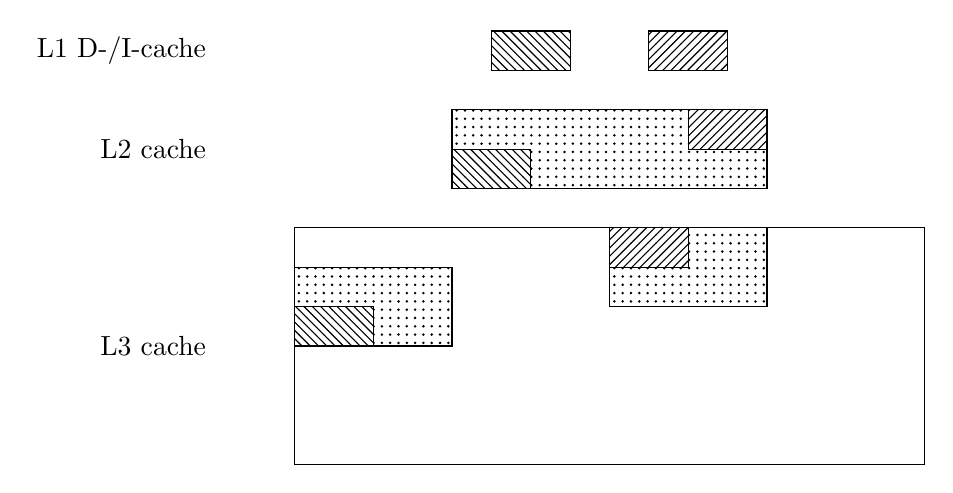
\begin{tikzpicture}

  \tikzstyle{rectangle} = [draw=black, shape=rectangle, inner sep = 1pt];

  % picture
  % L1I and L1D cache
  \begin{scope}[yshift=3.5cm, xshift=2.5cm]
    \draw [pattern=north west lines] (0,0) -- (0,.5) -- (1,.5) --
    (1,0) -- cycle;
    \draw [pattern=north east lines] (2,0) -- (2,.5) -- (3,.5) --
    (3,0) -- cycle;
  \end{scope}

  % L2 cache
  \begin{scope}[yshift=2cm, xshift=2cm]
    \draw [pattern=dots] (1,0) -- (4,0) -- (4,.5) -- (3,.5)
    -- (3,1) -- (0,1) -- (0,.5) -- (1,.5) -- cycle;
    \draw [pattern=north west lines] (0,0) -- (0,.5) -- (1,.5) --
    (1,0) -- cycle;
    \draw [pattern=north east lines] (3,0.5) -- (3,1) -- (4,1) --
    (4,0.5) -- cycle;
  \end{scope}
  
  % L3 cache
  \begin{scope}
    \draw (0,-1.5) -- (8,-1.5) -- (8,1.5) -- (0,1.5) -- cycle;
    \draw [pattern=dots] (0,.5) -- (0,1) -- (2,1) -- (2,0) -- (1,0)
    -- (1,.5) -- cycle;
    \draw [pattern=dots] (5,1.5) -- (6,1.5) -- (6,.5) -- (4,.5) -- (4,1) -- (5,1) --
    cycle;
    \draw [pattern=north west lines] (0,0) -- (0,.5) -- (1,.5) --
    (1,0) -- cycle;
    \draw [pattern=north east lines] (4,1) -- (4,1.5) -- (5,1.5) --
    (5,1) -- cycle;

  \end{scope}

  \node [draw=none, anchor=east] at (-1,0) {L3 cache};
  \node [draw=none, anchor=east] at (-1,2.5) {L2 cache};
  \node [draw=none, anchor=east] at (-1,3.75) {L1 D-/I-cache};

\end{tikzpicture}


\end{document}
